\documentclass{lecture}

\institute{Applied and Computational Mathematics}
\title{Vorlesung 3}
\author{Joshua Feld, 406718}
\course{Mathematische Grundlagen IV}
\professor{Torrilhon \& Berkels}
\semester{Sommersemester 2022}
\program{CES (Bachelor)}

\begin{document}
    \maketitle

    \begin{proof}
        Mit Lemma 2 aus Vorlesung 1 ergibt sich
        \begin{align*}
            T_n\parentheses*{y; x_k} &= \sum_{j = 0}^{n - 1}d_j\parentheses*{y}e^{i\frac{2\pi jk}n}\\
            &= \frac{1}{n}\sum_{j = 0}^{n - 1}\parentheses*{\sum_{l = 0}^{n - 1}y_l e^{-ijx_l}}e^{i\frac{2\pi jk}{n}}\\
            &= \sum_{l = 0}^{n - 1}y_l\frac{1}{n}\sum_{j = 0}^{n - 1}e^{-i\frac{2\pi j\parentheses*{l - k}}{n}}\\
            &= \sum_{l = 0}^{n - 1}y_l\delta_{l - k, 0} = y_k.
        \end{align*}
        Angenommen \(T \in \mathcal{T}_n\) erfüllt ebenfalls die Interpolationsbedingungen.
        Dann hat \(T - T_n\parentheses*{y; \cdot} \in \mathcal{T}_n\) \(n\) verschiedenen Nullstellen, denn für \(k \in \braces*{0, \ldots, n - 1}\) gilt
        \[
            T\parentheses*{x_k} - T_n\parentheses*{y; x_k} = y_k - y_k = 0.
        \]
        Aus Theorem 1 (ii) aus der ersten Vorlesung folgt, dass \(T - T_n\parentheses*{y; \cdot}\) das Nullpolynom ist, d.h. es gilt \(T = T_n\parentheses*{y; \cdot}\).
    \end{proof}


    \section*{Diskrete Fourier-Transformation}

    \begin{definition}
        Wir bezeichnen den Vektor
        \[
            \hat{y} := d\parentheses*{y} := \parentheses*{d_0\parentheses*{y}, \ldots, d_{n - 1}\parentheses*{y}}^T \in \C^n
        \]
        als die \emph{diskrete Fourier-Transformierte} von \(y\).
        Die Abbildung \(\mathcal{F}: \C^n \to C^n, y \mapsto \hat{y}\) heißt \emph{diskrete Fourier-Transformation (DFT)}.
        Die Komponenten von \(\hat{y}\) bezeichnen wir auch mit \(\hat{y}\).
    \end{definition}

    \begin{remark}
        Da die DFT linear ist, lässt sie sich als Matrix darstellen.
        Sei dazu \(B = \parentheses*{b^0 | \cdots | b^{n - 1}} \in \C^{n \times n}\) die Matrix mit den Spalten
        \[
            b^j = \parentheses*{e^{-\frac{2\pi ijk}{n}}}_{k = 0}^{n - 1} \equiv \parentheses*{1, e^{-\frac{2\pi ij}{n}}, \ldots, e^{-\frac{2\pi ij\parentheses*{n - 1}}{n}}}^T \in C^n.
        \]
        Dann gilt \(\hat{y} = \frac{1}{n}By\), also ist \(\frac{1}{n}B\) die Matrixdarstellung der DFT.
        Die Matrix \(B\) ist voll besetzt und wird damit in der Praxis nicht aufgestellt.
        Sie erlaubt es aber sehr einfach die inverse DFT herzuleiten.
    \end{remark}

    \begin{theorem}
        Die Menge der Vektoren \(\braces*{b^0, \ldots, b^{n - 1}}\) bildet eine Orthogonalbasis des \(\C^n\) bzgl. des unitären Standardskalarproduktes \(\angles*{\cdot, \cdot}: \C^n \times C^n \to \C\).
        Genauer gilt
        \[
            \angles*{b^k, b^l} = n\delta_{k, l}, \quad k, l \in \braces*{0, \ldots, n - 1}.
        \]
        Insbesondere gilt \(\parentheses*{\frac{1}{n}B}^{-1} = \overline{B}^T\), d.h. die Inverse der DFT ist
        \[
            y_j = \sum_{k = 0}^{n - 1}\hat{y}_k e^{\frac{2\pi ijk}{n}}, \quad j = 0, \ldots, n - 1.
        \]
    \end{theorem}

    \begin{proof}
        Die Orthogonalität folgt mithilfe von Lemma 2 aus der ersten Vorlesung
        \[
            \angles*{b^k, b^l} = \sum_{j = 0}^{n - 1}b_j^k \overline{b_j^l} = \sum_{j = 0}^{n - 1}e^{-\frac{2\pi ikj}{n}}e^{\frac{2\pi ilj}{n}} = \sum_{j = 0}^{n - 1}e^{-\frac{2\pi i\parentheses*{k - l}j}{n}} = n\delta_{k - l, 0} = n\delta_{k, l}.
        \]
        Aus \(\angles*{b^k, b^l} = n\delta_{k, l}\) folgt \(\parentheses*{\overline{B}^T B} = nI_n\) und daraus \(\parentheses*{\frac{1}{n}B}^{-1} = \overline{B}^T\).
        Für die adjungierte Matrix \(\overline{B}^T\) gilt
        \[
            \parentheses*{\overline{B}^T}_{k, l} = \parentheses*{\overline{B}}_{l, k} = \overline{b_l^k} = e^{\frac{2\pi ikl}{n}}.
        \]
        Daraus folgt direkt die Darstellung der Inversen.
    \end{proof}

    \begin{remark}
        Mit anderen Worten ist die DFT ein Basiswechsel von der kanonischen Basis in die Basis \(\overline{b}^0, \ldots, \overline{b}^{n - 1}\), denn es gilt
        \[
            y = \sum_{k = 0}^{n - 1}\hat{y}_k\overline{b^k}.
        \]
        Wir bezeichnen die \emph{inverse (diskrete) Fourier-Transformierte} von \(y\) mit \(\check{y}\), bzw. die \emph{inverse (diskrete) Fourier-Transformation} mit \(\mathcal{F}^{-1}: \C^n \to \C^n\).
        Es gilt also \(\check{y} = \mathcal{F}^{-1}\parentheses*{y}\).
    \end{remark}

    \begin{remark}
        Seien \(f: \brackets*{0, 2\pi} \to \C\) und \(y_k := f\parentheses*{x_k}\).
        Neben der Interpretation der Formel für \(d_j\parentheses*{y}\) als Quadraturformel für die Fourier-Koeffizienten gibt es weitere Analogien zur Fourier-Teilsumme.
        Für Funktionen \(f, g: \brackets*{0, 2\pi} \to \C\) definieren wir das (diskrete) innere Produkt \(\angles*{\cdot, \cdot}_n\) als
        \[
            \angles*{f, g}_n := \frac{1}{n}\sum_{l = 0}^{n - 1}f\parentheses*{x_l}\overline{g\parentheses*{x_l}}.
        \]
        Mit den Grundschwingungen \(e_k\) gilt dann
        \[
            d_j\parentheses*{y} = \frac{1}{n}\sum_{l = 0}^{n - 1}y_l e^{-ijx_l} = \frac{1}{n}\sum_{l = 0}^{n - 1}f\parentheses*{x_l}\overline{e_j\parentheses*{x_l}} = \angles*{f, e_j}_n = \angles*{T_n\parentheses*{y; \cdot}, e_j}_n.
        \]
        Mehr noch: Es gilt
        \[
            \angles*{e_j, e_k}_n = \frac{1}{n}\sum_{l = 0}^{n - 1}e_j\parentheses*{x_l}\overline{e_k\parentheses*{x_l}} = \frac{1}{n}\sum_{l = 0}^{n - 1}e^{ijx_l}\overline{e^{ikx_l}} = \frac{1}{n}\sum_{l = 0}^{n - 1}\overline{b_l^j}\overline{\overline{b_l^k}} = \frac{1}{n}\overline{\parentheses*{b^j, b^k}} = \delta_{j, k}.
        \]
        Also sind die \(e_j\) nicht nur bezüglich des kontinuierlichen inneren Produkts \(\angles*{\cdot, \cdot}\), sondern auch bezüglich des diskreten Analogons \(\angles*{\cdot, \cdot}_n\) ein Orthonormalsystem.
        Das trigonometrische Polynom ist bezüglich des diskreten inneren Produkts eine Orthogonalprojektion.
    \end{remark}

    \begin{example}
        Wir betrachten den Fall \(n = 4\) und die folgenden Daten
        \begin{center}
            \begin{tabular}{lcccc}
                \toprule
                \(x_k\) & \(0\) & \(\frac{\pi}{2}\) & \(\pi\) & \(\frac{3\pi}{2}\)\\
                \midrule
                \(y_k\) & \(2\) & \(0\) & \(2\) & \(0\)\\
                \bottomrule
            \end{tabular}
        \end{center}
        Die zugehörige Einheitswurzel ist \(\varepsilon_4 = e^{-\frac{i\pi}{2}} = -i\).
        Weiterhin gilt:
        \begin{align*}
            d_0\parentheses*{y} &= \frac{1}{4}\sum_{l = 0}^3 y_l \cdot 1 = \frac{1}{4}\parentheses*{2 + 0 + 2 + 0} = 1,\\
            d_0\parentheses*{y} &= \frac{1}{4}\sum_{l = 0}^3 y_l\parentheses*{-i}^l = \frac{1}{4}\parentheses*{2 \cdot 1 + 0 \cdot \parentheses*{-i} + 2 \cdot \parentheses*{-1} + 0 \cdot i} = 0,\\
            d_1\parentheses*{y} &= \frac{1}{4}\sum_{l = 0}^3 y_l\parentheses*{-i}^{2l} = \frac{1}{4}\parentheses*{2 \cdot 1 + 0 \cdot \parentheses*{-i}^2 + 2 \cdot \parentheses*{-1}^4 + 0 \cdot \parentheses*{-i}^6} = 1,\\
            d_2\parentheses*{y} &= \frac{1}{4}\sum_{l = 0}^3 y_l\parentheses*{-i}^{3l} = \frac{1}{4}\parentheses*{2 \cdot 1 + 0 \cdot \parentheses*{-i}^3 + 2 \cdot \parentheses*{-1}^6 + 0 \cdot \parentheses*{-i}^9} = 0.
        \end{align*}
        Damit folgt
        \[
            T_4\parentheses*{y; x} = \sum_{j = 0}^3 d_j\parentheses*{y}e^{ijx} = 1 \cdot e^0 + 1 \cdot e^{2ix} = 1 + \cos\parentheses*{2x} + i\sin\parentheses*{2x}.
        \]
        Der Real- und Imaginärteil dieses trigonometrischen Interpolationspolynoms ist in der folgenden Abbildung zusammen mit den Daten \(y\) skizziert.
        \begin{center}
            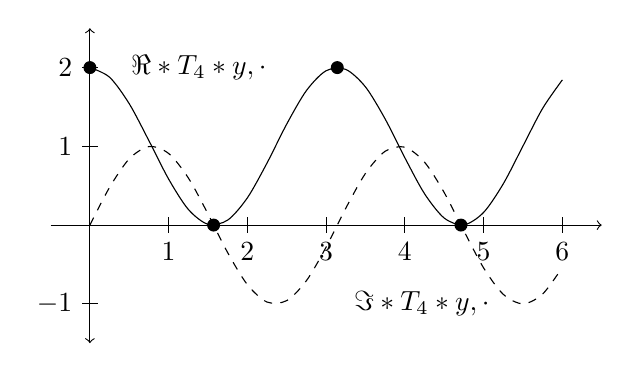
\begin{tikzpicture}
                \draw[<->] (0,-1.5) -- (0,2.5);
                \draw[->] (-.5,0) -- (6.5,0);
                \draw[domain=0:6,smooth,variable=\x] plot ({\x}, {1 + cos(2*\x r)});
                \draw[dashed,domain=0:6,smooth,variable=\x] plot ({\x}, {sin(2*\x r)});
                \draw[fill=black] (0,2) circle (.75mm);
                \draw[fill=black] (pi/2,0) circle (.75mm);
                \draw[fill=black] (pi,2) circle (.75mm);
                \draw[fill=black] (3*pi/2,0) circle (.75mm);
                \draw (1,.1) -- (1,-.1) node[below] {\(1\)};
                \draw (2,.1) -- (2,-.1) node[below] {\(2\)};
                \draw (3,.1) -- (3,-.1) node[below] {\(3\)};
                \draw (4,.1) -- (4,-.1) node[below] {\(4\)};
                \draw (5,.1) -- (5,-.1) node[below] {\(5\)};
                \draw (6,.1) -- (6,-.1) node[below] {\(6\)};
                \draw (.1,-1) -- (-.1,-1) node[left] {\(-1\)};
                \draw (.1,1) -- (-.1,1) node[left] {\(1\)};
                \draw (.1,2) -- (-.1,2) node[left] {\(2\)};
                \node[anchor=east] at (5.2,-1) {\(\Im\parentheses*{T_4\parentheses*{y, \cdot}}\)};
                \node[anchor=west] at (.4,2) {\(\Re\parentheses*{T_4\parentheses*{y, \cdot}}\)};
            \end{tikzpicture}
        \end{center}
    \end{example}

    \begin{remark}
        Es gibt diverse Varianten der diskreten Fourier-Transformation, u.a. die reelle trigonometrische Interpolation, die wir kurz darstellen wollen.

        Zunächst stellt sich die Frage nach einem geeigneten Raum um reelle Werte \(y_k\) mit reellen Funktionen zu interpolieren.
        Als Ausgangspunkt betrachten wir hierzu Real- und Imaginärteil der Grundschwingungen \(e_j\), also \(\phi_j := \Re\parentheses*{e_j} = \cos\parentheses*{j\cdot}\) und \(\psi_j := \Im\parentheses*{e_j} = \sin\parentheses*{j\cdot}\).
        Man rechnet leicht nach, das diese orthogonal bzgl. des Skalarproduktes \(\angles*{\cdot, \cdot}\) sind.
        Zusammen mit \(\phi_0 \equiv 1\) und \(\psi_0 \equiv 0\) führt das auf den reellen Raum
        \[
            \hat{\mathcal{T}}_{2p + 1} = \braces*{\alpha_0 + \sum_{j = 1}^p\parentheses*{\alpha_j\cos\parentheses*{jx} + \beta_j\sin\parentheses*{jx}} : \alpha_j, \beta_j \in \R} = \setspan\braces*{\phi_0, \ldots, \phi_p, \psi_1, \ldots, \psi_p}.
        \]
        Aus der Orthogonalität der aufspannenden Funktionen folgt \(\dim\hat{\mathcal{T}}_{2p + 1} = 2p + 1\).

        Zu gegebenen Werten \(y_k \in \R, k = 0, \ldots, n - 1\), sowie den Stützstellen \(x_k = \frac{2\pi k}{n}\) suchen wir nun ein \(\hat{T}_n \in \hat{\mathcal{T}}_n\), so dass gilt
        \[
            \hat{T}_n\parentheses*{x_k} = y_k, \quad k = 0, \ldots, n - 1.
        \]
        Wir nehmen dabei an, dass \(n\) ungerade ist, d.h. \(n = 2p + 1\) mit \(p \in \N_0\).

        Dieses Problem kann sehr ähnlich wie im komplexen Fall gelöst werden.
        Wir setzen
        \[
            A_j\parentheses*{y} := \frac{2}{n}\sum_{l = 0}^{n - 1}y_l\cos\parentheses*{jx_l} \quad \text{und} \quad B_j\parentheses*{y} := \frac{2}{n}\sum_{l = 0}^{n - 1}y_l\sin\parentheses*{jx_l}.
        \]
        Dann erfüllt
        \[
            \hat{T}_n\parentheses*{y; x} = \frac{1}{2}A_0\parentheses*{y} + \sum_{j = 1}^{\frac{n - 1}{2}}\parentheses*{A_j\parentheses*{y}\cos\parentheses*{jx} + B_j\parentheses*{y}\sin\parentheses*{jx}}
        \]
        die Interpolationsbedingungen \(\hat{T}_n\parentheses*{y; x_k} = y_k, k = 0, \ldots, n - 1\).
        In der Tat ist auch hier Lemma 2 aus der ersten Vorlesung der Schlüssel um diese Aussage zu zeigen.
        Um das Lemma anwenden zu können nutzt man die Identitäten
        \[
            \cos\parentheses*{x} = \frac{1}{2}\parentheses*{e^{ix} + e^{-ix}} \quad \text{und} \quad \sin\parentheses*{x} = \frac{1}{2i}\parentheses*{e^{ix} - e^{-ix}}.
        \]
        Die Koeffizienten \(A_j\parentheses*{y}\) und \(B_j\parentheses*{y}\) lassen sich effizient mit der diskreten Fourier-Transformation berechnen.
        Hierzu wird aus dem reellen Vektor \(y\) ein komplexer Vektor halber Länge konstruiert, auf den man die Fourier-Transformation anwendet.
        Hieraus kann man dann die gesuchten Koeffizienten mit sehr geringem Aufwand berechnen.
    \end{remark}


    \section*{Schnelle Fourier-Transformation}

    Nun zur oft erwähnten schnellen Fourier-Transformation (Fast Fourier Transform, FFT).

    \begin{remark}
        Wir erinnern uns, dass die Koeffzienten gegeben sind durch
        \[
            d_j\parentheses*{y} = \frac{1}{n}\sum_{l = 0}^{n - 1}y_l e^{-i\frac{2\pi jl}{n}} = \frac{1}{n}\sum_{l = 0}^{n - 1}y_l\varepsilon_n^{jl}, \quad j = 0, \ldots, n - 1,
        \]
        mit der \(n\)-ten Einheitswurzel \(\varepsilon_n\).
        Naiv ausgeführt erfordert die diskrete Fourier-Transformation also die Bestimmung von \(n\) Koeffizienten, deren Berechnung jeweils \(O\parentheses*{n}\) Operationen erfordert, mithin insgesamt einen Aufwand von \(O\parentheses*{n^2}\).
        Man sieht sehr schnell, dass die Behandlung von Datensätzen mit \(n = 10^6\) auf normalen Rechnern unmöglich wird (\(1\,\text{GFLOP} = 10^9\,\text{Operationen}\)).
        Eine solche Datenmenge ist jedoch alles andere als ungewöhnlich.
        Bei einer Audio-Samplingrate von \(48\sis{\kilo\hertz}\), d.h. \(48000\) Datenpunkten pro Sekunde entsprechen 5 Minuten schon \(1,44 \cdot 10^7\) Datenpunkten.
        Durch geschicktes Rechnen mit komplexen Zahlen lässt sich der Aufwand auf \(O\parentheses*{n\log n}\), also praktisch lineares Verhalten, senken.
        Erst dies macht Audio- und Videokompression möglich.
        Die FFT gilt daher zurecht als einer der wichtigsten Algorithmen unserer Zeit.
    \end{remark}
\end{document}
